\documentclass[runningheads]{llncs}

%---- Codierung----%
\usepackage[utf8]{inputenc} 
%\usepackage[T1]{fontenc}
\usepackage{graphicx}
%\usepackage{url}
\usepackage{llncsdoc}
%----- Mathematischer Zeichenvorrat---%
%\usepackage{amsmath}
%\usepackage{amssymb}
%\usepackage{enumerate}
\usepackage{proof}
\usepackage{mathpartir}
% fuer die aktuelle Zeit 
%\usepackage{scrtime}
%\usepackage{listings}
%\usepackage{subfigure}
\usepackage{hyperref}

%referenzieren von Abbildungen
\usepackage[figure]{hypcap}
\setcounter{tocdepth}{3}
\setcounter{secnumdepth}{3}

% Syntax highlighting von Java Code
\usepackage{listings}
\usepackage{color}
 
\definecolor{dkgreen}{rgb}{0,0.6,0}
\definecolor{gray}{rgb}{0.5,0.5,0.5}
\definecolor{mauve}{rgb}{0.58,0,0.82}

\lstset{frame=tb,
  language=Java,
  aboveskip=3mm,
  belowskip=3mm,
  showstringspaces=false,
  columns=flexible,
  basicstyle={\small\ttfamily},
  numbers=left,
  numberstyle=\tiny\color{gray},
  keywordstyle=\color{blue},
  commentstyle=\color{dkgreen},
  stringstyle=\color{mauve},
  breaklines=true,
  breakatwhitespace=true,
  tabsize=3,
  escapechar=@
}
 
\usepackage{graphicx}
\begin{document}

\mainmatter
\title{Taint Analyse für Android Apps} 
\titlerunning{Taint Analyse für Android Apps}
\author{Thomas Czogalik}
\authorrunning{Desaster in der Software-Sicherheit (WiSe15/16)}
\institute{Betreuer: Simon Greiner}
\date{31.03.2016}
\maketitle

\section{Motivation} 
Computersysteme sind heutzutage in nahezu allen Bereichen unseres Lebens intigriert. Datenlecks können deshalb fatale folgen haben. Besonders Smartphones verwalten und verarbeiten viele vertauliche und private Daten und komunizieren dabei oft mit der Außenwelt. Im Februar 2015 befanden sich im Google Play Store ca. 1.4 Millionen Apps (\ref{fig:playstore}). Diese Apps sind jedem zugänglich, der auf seinem mobilen Gerät das Betriebssystem Android installiert hat. Bei so einer großen Anzahl Apps bietet der Google Play Store eine große Angriffsfläche für Angreifer die Datenlecks ausnutzen. \\
Betrachten wir den folgenden Ausschnitt aus einem Java Programm in Abbildung \ref{fig:sql_code}. In Zeile \ref{sql:connection} wird zunächst eine Verbindung zu einer Datenbank hergestellt. In den nächsten beiden Zeilen \ref{sql:createStmt} und \ref{sql:createBr} werden ein Statement Objekt und ein BufferdReader Objekt erstellt. In Zeile \ref{sql:name} wird eine Benutzereingabe eingelesen und dem String name zugewiesen. In Zeile \ref{sql:sql} wird der String name in einen vorbereiteten SQL String eingesetzt. Schließlich wird in Zeile \ref{sql:execute} das Statement mit dem sql String ausgeführt. 
\\Durch folgende Benutzereingabe: "\emph{foo; DROP TABLE users}" kann die Datenbank \emph{users} gelöscht werden. Es können aber auch mit einem beliebigen SELECT Statement Daten aus der Datenbank geholt werden. 
\\Durch eine Überprüfung der Benutzereingabe hätte man diesen Fehler vermeiden können. Es ist aber nicht immer so einfach Datenlecks im Code zu finde. 
Deshalb wäre es hilfreich, wenn man den Fluss sensitiver Daten nachvollziehen könnte. Dies ist mithilfe einer Taint Analyse möglich. \\
Im folgenden wird zunächst auf die Grundlagen der Taint Analyse eingegangen um sie dann anschließend Formal darzustellen [\ref{sec:taintAnalyse}]. Außerdem werden Eigenschaften für die Taint Analyse vorgestellt, die zur einer besseren Präzision führen [\ref{sec:precision}]. Im Anschluß wird auf die Probleme bei Android eingegangen die bei einer Taint Analyse auftretten [\ref{sec:android}]. Scließlich wird FlowDroid vorgestellt, das sich dieser Probleme annimmt und versucht eine präzise Taint Analyse für Android Apps bereitzustellen [\ref{sec:flowdroid}].
 
\begin{figure}
\lstinputlisting[language=Java]{code/sql_example.java}
\caption{Beispiel bei dem SQL Injections möglich sind}
\label{fig:sql_code}
\end{figure}

\begin{figure}[htp]
\centering
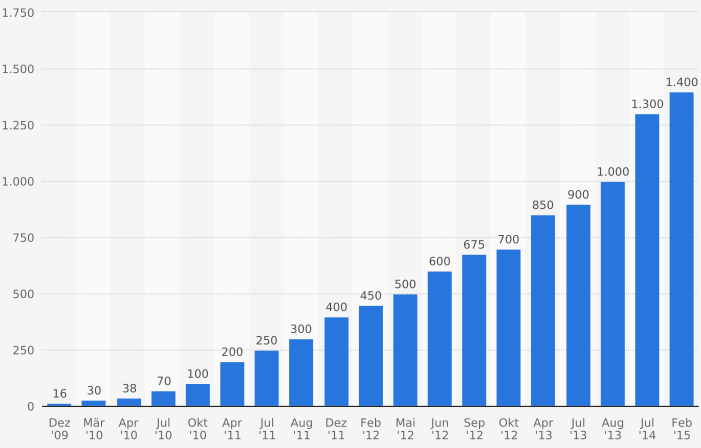
\includegraphics[scale=0.60]{img/playstore.png}
\caption{Anzahl der verfügbaren Apps im Google Play Store von Dezember 2009 bis Februar 2015 (in 1.000), aus \cite{playstore}}
\label{fig:playstore}
\end{figure} 

\section{Taint Analyse}\label{sec:taintAnalyse}
Die Taint Analyse ist eine Datenflussanalyse. Man unterscheidet zwischen statischer und dynamischer Taint Analyse. Bei einer statische Analyse wird der Quelltext einer Reihe formaler Prüfungen unterzogen. Der Vorteil dabei ist, dass das Kompilat nicht ausgeführt werden muss um gegensatz zur dynamischen Analyse, die ein laufendes Programm voraussetzt. Dies ist hilfreich, da heutige Malware erkennen kann ob sie überwacht wird und ihr Verhalten der Situation anpasst. \\
Im folgenden wird sich auf die statische Taint Analyse beschränkt.\\
Die Taint Analyse nimmt zunächst an, dass jede von außen veränderbare Variable ein Sicherheitsrisiko birgt. Ihr Ziel ist es, die Software gegen externe Angriffe, sowie interne Risiken abzusichern. Dazu sucht die Taint Analyse nach Datenflüssen von möglichen tainted Sources zu einem Sink. Als Source wird eine Funktion bezeichnet, die Quelle sensitiver Daten ist. Ein Sink ist eine Funktion, die Daten möglicherweiese an nicht vertrauenswürdige Beobachter weitergibt. Welche Funktionen im einzelnen Sources und Sinks sind, muss vor dem ausführen der Taint Analyse spezifiziert werden. In dem Beispiel aus Abbildug \ref{fig:sql_code} wäre die Funktion \emph{readLine()} eine Source, da Daten von außen eingeführt werden (Benutzereingabe) und die Funktion \emph{executeQuery(sql : String)} ein Sink, da hier möglicherweise sensitive Daten weitergegeben werden.
\subsection{Formal}
Im Folgendem wird die Taint Analyse mithilfe von Schlussregeln formalisiert(\ref{fig:schlussregeln}). Die SOURCE Regel beschreibt die Einfuhr von tainted Daten durch einen Source. \emph{src(m,l)} bedeutet, dass dem Parameter \emph{m} Daten aus einer Source zugewiesen werden mit dem Namen \emph{l}. \emph{l} ist der Name einer Source, die aus einem Source-Label-Set stammt. Wenn \emph{m} auf einen Objektrepräsentanten \emph{o} zeigt, ist \emph{o} durch die Source \emph{l} tainted. \\Als Objektrepräsentant wird ein Objekt im Sinne der Analyse bezeichnet. Da nicht sicher ist auf wieviele Objekte tatsächlich zur Laufzeit ein Zeiger zeigt, fasst man diese Menge zusammen und wählt einen Objekträpresentanten. 
\\Die zweite Regel TRANSFER beschreibt die Übertragung von tainted Daten. \emph{transfer(m,n)} bedeutet, dass Daten vom Parameter \emph{m} zu \emph{n} übertragen werden. Wenn außerdem der Objektrepräsentant \emph{o1} von einer Source \emph{l} tainted ist und \emph{m} auf \emph{o1} und \emph{n} auf ein \emph{o2} zeigt, dann ist auch \emph{o2} durch \emph{l} tainted.
\\Die letzte Regel SOURCE beschreibt den Datenfluss von verschmutzen Daten zu einem Sink. Wenn der  Objektrepräsentant \emph{o} durch eine Source \emph{so} tainted ist und die Variable \emph{m}, die auf \emph{o} zeigt einem Sink mit dem Namen \emph{si} übergeben wird, dann gibt es einen Datenfluss von der Source \emph{so} zum Sink \emph{si}. \emph{si} ist dabei der Name eines Sinks aus einem Sink-Label-Set. 
\\Mit diesen drei Regeln kann man eine Taint Analyse durchführen indem man diese solange immer wieder ausführt, bis sich am Ergebniss nichts mehr ändert.
\begin{figure}
\begin{mathpar}
\infer[(SOURCE)] {tainted(o, l)}{src(m,l)\\ m \rightarrow o}\\\\
\infer[(TRANSFER)] {tainted(o_2, l)}{tainted(o_1,l)\\ m \rightarrow o_1 \\ n \rightarrow o_2 \\ transfer(m,n)}\\\\
\infer[(SOURCE)] {flow(so, si)}{tainted(o,so)\\ m \rightarrow o \\ sink(m,si)} 
\end{mathpar}
\caption{Schlussregeln für die Taint Analyse}
\label{fig:schlussregeln}
\end{figure}

\subsubsection{Beispiel}
Im folgenden wird dargestellt wie die Anwendung der Regeln auf das Beispiel aus Abbildung \ref{fig:sql_code} aussieht. 
\\Zunächst müssen die Sources und Sinks definiert werden. Dazu wird die Funktion \emph{readLine} aus Zeile vier in das Source-Label-Set eingefügt. In das Sink-Label-Set wird die Funktion \emph{executeQuery} aus Zeile sechs eingefügt. Die Taint Analyse wird zunächst die SOURCE Regel in Zeile vier anwenden, da dort Daten aus einer Source dem String \emph{name} zugewiesen werden. Somit wird der String \emph{name} als tainted markiert. Als nächstes wird die TRANSFER Regel in Zeile fünf angewendet. Hier werden Daten vom String "name" zum String \emph{sql} übertragen. Deshalb wird auch hier der String \emph{sql} als tainted markiert. Schließlich wird in Zeile sechs die SINK Regel angewendet. Hier wird der String \emph{sql} in den Sink \emph{executeQuery} übergeben. Da \emph{sql} tainted ist, wird der Sink \emph{executeQuery} auch als tainted markiert. Somit wurde ein tainted Datenfluss von der Source \emph{readLine} zum Sink \emph{executeQuery} gefunden.

\subsection{Sanitization}
Mithilfe von Sanitization Funktionen lassen sich Code Injections verhindern. Als Code Injection bezeichnet man das ausnutzen eines Programmfehlers indem man Code in das Program einschleust.
\\In Abbildung \ref{fig:sql_code} würde zum Beispiel die Funktion \emph{onlyLetters(s : String) : String} die Benutzereingabe als Parameter entgegen nehmen, alle nicht Buchstaben aus der Eingabe entfernen und einen String zurückgeben, der nur aus Buchstaben besteht. Einige Programmiersprachen bieten solche Säuberungsfunktionen an. PHP hat zum Beispiel die Funktion \emph{htmlentities}. Diese Funktion konvertiert Zeichen, die in HTML besondere Bedeutung haben in ihre HTML Instanzen. Aus dem Zeichen '\textless' wird "\&lt;".\\
Eine Taint Analyse die Sanitization unterstützt, hat den Vorteil, dass gesäuberte Werte nicht länger als tainted angesehen werden und nicht mehr als tainted verbreitet werden.

\section{Präzision}\label{sec:precision}
Eine gute Analyse sollte in der Lage sein keine false-positives zu finden. Dadurch wird zum einen die manuelle Aussortierung dieser durch den Benutzer vermieden und zum anderen die Präzision der Analyse erhöht. Dabei ist ein false-positives ein Ergebni das anzeigt, dass eine bestimmte Voraussetzung erfüllt ist, obwohl dies nicht der Fall ist. Eine Analyse die eine oder mehrere der folgenden Eigenschaften implementiert hat den Vorteil, dass weniger false-positives gefunden werden.

\subsection{Fluss-Sensitivität}
Eine Analyse die Fluss-Sensitiv ist, beachtet die Reihenfolge der Programmbefehle.
In Abbildung \ref{fig:fluss_code} wird dem String \emph{s} in Zeile \ref{flow:s} zunächst ein harmloser Wert zugewiesen. Danach wird dieser String in Zeile \ref{flow:sink} einem Sink übergeben. Im Anschluss werden in Zeile \ref{flow:source} dem String \emph{s} tainted Daten aus einem Source zugewiesen. \\
Eine Fluss-Sensitive Analyse wird den Sink in Zeile \ref{flow:sink} nicht als tainted markieren, da sie die Reihenfolge der Programmbefehle beachtet. 

\begin{figure}
\lstinputlisting[language=Java]{code/flow_sensitive_example.java}
\caption{Fluss-Sensitivität}
\label{fig:fluss_code}
\end{figure}

\subsection{Kontext-Sensitivität}
Ist eine Analyse Kontext-Sensitiv, beachtet sie den Kontext des Aufrufs. Dies bedeutet, dass eine solche Analyse zu dem Aufrufer einer Funktion zurück springen kann und somit den genauen Funktionsaufrufer bestimmen kann, während eine Analyse die nicht Kontext-Sensitiv ist alle möglichen Aufrufer berücksichtigen muss.
In Abbildung \ref{fig:context_code} werden den beiden Strings \emph{s1} und \emph{s2} die Rückgabe der Funktion \emph{id(s : String) : String} zugewiesen. Die Funktion \emph{id} ist dabei die Identitätsfunktion. Nun wird \emph{id} einmal in Zeile \ref{context:s1} mit tainted Daten ausgeführt und \emph{s1} zugewiesen und noch einmal in Zeile \ref{context:s2} mit einem harmlosen String und \emph{s2} zugewiesen. Schließlich wird \emph{s2} dem sink in Zeile \ref{context:sink} übergeben. Eine Kontext-Sensitive Analyse kann hier zwischen den beiden Aufrufen in Zeile \ref{context:s1} und \ref{context:s2} unterscheiden und wird den Sink in Zeile \ref{context:sink} nicht als tainited markieren.
 
\begin{figure}
\lstinputlisting[language=Java]{code/context_sensitive_example.java}
\caption{Kontext-Sensitivität}
\label{fig:context_code}
\end{figure}

\subsection{Objekt-Sensitivität}
Die Objekt-Sensitivität ist ein Subtyp der Kontext-Sensitivität. Eine Objekt-Sensitive Analyse beachtet nämlich den Kontext des aufrufenden Objekts. Das heißt, dass zu dem Objekt zurück gesprungen werden kann, dass eine Methode aufruft.
In Abbildung \ref{fig:object_code} werden zunächst zwei Foo Objekte \emph{o1} und \emph{o2} erstellt. Die Klasse Foo  besteht aus einem String mit Namen \emph{value} und einer \emph{getValue() : String} Methode, die \emph{value} zurückgibt. In Zeile \ref{object:o1} und \ref{object:o2} wird \emph{o1} ein harmloser String übergeben und \emph{o2} tainted Daten aus einer Source. Im Anschluss wird in Zeile \ref{object:sink} die Funktion \emph{getValue} auf \emph{o1} aufgerufen und der Rückgabewert einem Sink übergeben. Eine Objekt-Sensitive Analyse kann zwischen den beiden Objekten \emph{o1} und \emph{o2} unterscheiden und markiert den Sink in Zeile \ref{object:sink} nicht als tainted. 

\begin{figure}
\lstinputlisting[language=Java]{code/object_sensitive_example.java}
\caption{Objekt-Sensitivität}
\label{fig:object_code} 
\end{figure}

\subsection{Feld-Sensitivität}
Eine Feld-Sensitive Analyse kann Felder einer Klasse einzelnd betrachten. Macht eine Analyse dies nicht, werden die Felder zu ihrem Basis Objekt zurückgeführt.
In Abbildung \ref{fig:field_code} wird in Zeile \ref{field:o} zunächst ein Foo Objekt \emph{o} erstellt. Die Klasse Foo enthält hier 2 Felder \emph{field1} und \emph{field2}. In Zeile \ref{field:f1} und \ref{field:f2} wird \emph{field1} ein harmloser String zugewiesen während \emph{field2} tainted Daten zugewiesen werden. Schließlich wird \emph{field1} in einen Sink in Zeile \ref{field:sink} übergeben. Bei einer Feld-Sensitiven Analyse wird hier der Sink nicht als tainted markiert.

\begin{figure}
\lstinputlisting[language=Java]{code/field_sensitive_example.java}
\caption{Feld-Sensitivität}
\label{fig:field_code}
\end{figure}

\section{Android}\label{sec:android}
%\subsection{Grundlagen}
Android ist sowohl ein Betriebssystem als auch eine Software-Platform für mobile Geräte. Es bietet Entwicklern eine Schnittstelle an, um auf verschiedene Systemfunktionalitäten des mobilen Gerätes zuzugreifen. Der Nutzerstandort ist zum Beispiel eine solche Funktionalität. Der Entwickler muss die von ihm genutzte Funktionalität in die \emph{AndroidManifest.xml} eintragen. Der Benutzer, der die App installieren möchte muss dieser die Berechtigung geben auf diese Funktionalitäten zugreifen zu dürfen. Werden die Berechtigungen verweigert, kann die App nicht installiert werden. Das Problem ist, dass oft zu viele Berechtigungen gefordert werden. Entweder aus Unkenntnis oder mit bösen Absichten. Außerdem sind viele Berechtigungen zu mächtig und können ausgenutzt werden. Eine social-network App zum Beispiel, möchte die Berechtigung\\\emph{android.permission.READ\_CONTACTS} um neue Freunde anhand der Email Adresse vorschlagen zu können. Sie kann aber mit dieser Berechtigung auch Telefonnummern und sonstige Kontaktdaten auslesen, auch wenn der Kontakt nicht bei dem Dienst angemeldet ist. Trojaner können dies ausnutzen. 
\\Um dem entgegenzuwirken kann man die Datenflüsse einer Android App mithilfe der Taint Analyse analysieren. Dabei gibt es einige Besonderheiten und 
\\Schwierigkeiten gegenüber anderen \emph{JAVA} Programmen. Eine Android App kann nämlich aus vier verschiedenen Komponenten bestehen.\\\\
\begin{tabular}{ll}
	Activity & Einzelner Screen, der für den Benutzer sichtbar ist\\
	Service & Eine Aktion die im Hintergrund abläuft\\
	Content Provider & Ist zuständig für das Speichern von Daten\\
	Broadcast Reciever & Wartet auf ein globales Ereignis und führt eine vordefinierte \\
	& Aktion aus\\\\
\end{tabular}
Aufgrund dieser Besonderheit entstehen bestimmte Probleme für eine Taint Analyse. Zum einen hat eine Android App keine zentrale \emph{main} Methode, sondern mehrere Einstiegspunkte. Eine App kann zum Beispiel aus drei Activities und einem Service bestehen. Es gibt zwar eine Haupt-Activity, aber welche Komponente als nächstes an die Reihe kommt ist im allgemeinen nicht bestimmbar, da es oft auf die Benutzereingabe ankommt. Außerdem haben die einzelnen Komponenten besonderes Verhalten. Sie können zum Beispiel gestartet und beendet werden oder angehalten werden, wenn der Speicher voll ist und fortgesetzt, wenn wieder Speicher frei ist. Somit entsteht ein komplizierter Lebenszyklus, mit dem die Taint Analyse umgehen muss. Außerdem muss vor der Analyse spezifiziert werden, was Sources und Sinks in Android sind.

\section{FlowDroid}\label{sec:flowdroid}
FlowDroid ist eine statische Taint Analyse die, Fluss-, Kontext-, Objekt- und Feld-Sensitiv ist \footnote{\url{https://github.com/secure-software-engineering/soot-infoflow-android/wiki}}.
Für die Sinks und Sources benutzt FlowDroid die Ausgabe des Tools SuSi. SuSi ist ein machine-learning Tool, dass vollautomatisch den Android Source Code analysiert und eine Liste von Sinks und Sources generiert. Außerdem wird vor der Analyse ein präziser Android Lebenszyklus modelliert.
\subsection{Lebenszyklus}
Aufgrund der vielen möglichen Einstiegspunkte bei einer Android App, wird bei FlowDroid zunächst eine dummy-main-Mehtode erstellt. Diese Methode wird individuell für jede App erstellt. Die dummy-main enthält nur Teile des Lebenszyklus die auch auftreten können. Um diese zu indentifizieren werden die XML Konfigurationsdateien und der Quellcode analysiert. Danach ruft die dummy-main-Methode nachheinander Teile des Zykluses auf.
\subsection{Evaluation}
Für die Evaluerung wurde die Testumgebung DroidBench \footnote{\url{https://github.com/secure-software-engineering/DroidBench}} verwenden. DroidBench enthielt zum damaliegen Zeitpunkt 39 Apps mit verschiedenen Analyse Problemen. Vergliechen wurde FlowDroid mit den beiden komerziellen Analyse Tools \emph{App Scan} von IBM und \emph{Fortify SCA} von HP. 
In dem Evaluierungsbogen (\ref{fig:eval}) ist zu erkennen, dass FlowDroid in den Kategorien \emph{Callbacks} und \emph{Lifecycle} deutlich besser ist, als die beiden anderen Tools. Dies ist auf die präzise Modelierung des Lebenszyklus zurückzuführen. In ein paar Tests schlägt FlowDroid aber auch fehl. Zum Beispiel findet FlowDroid keinen Fehler im \emph{IntentSink1} Test. Das liegt daran, dass in dem Test tainted Daten aus einer Komponente in die nächste übergeben werden und diese die Daten direkt wieder zurück schickt. FlowDroid verfolgt tainted Daten nur innerhalb von Komponenten. Deshalb schlägt der Test hier fehl. Ein weiterer Test der Fehlschlägt ist der \emph{StaticInitialization1} Test. Hier liegt der Grund in dem verwendeten Framework Soot. 
\\Soot ist ein Framework zum analysieren und transformieren von Java und Android Programmen. Es kann aus Java Code einen Call-Graphen generieren. Dabei geht Soot davon aus, dass die komplette statische Initialisierung zu beginn stattfindet, was in diesem Testfall nicht der Fall ist.
\\Im Ergebniss schneidet FlowDroid jedoch besser ab, als seine beiden Konkurenten. FlowDroid ist mit 86\% etwas besser beim Verhältnis zwischen gefunden Fehlern und false-positives (Precision p). Mit 93\% gegenüber 50\% und 61\% ist FlowDroid aber deutlich besser beim auffinden aller Fehler (Recall r).
\\Mit FlowDroid wurden zusätzlich die damals Top 500 Apps des Google Play Stores getestet. Dabei wurden in den meisten Apps ein Datenleck gefunden. 
\\Außerdem wurden 1000 Malware Apps des VirusShare Projects analysiert. Es wurden pro App ca. zwei Datenlecks gefunden.

\begin{figure}[htp]
\centering 
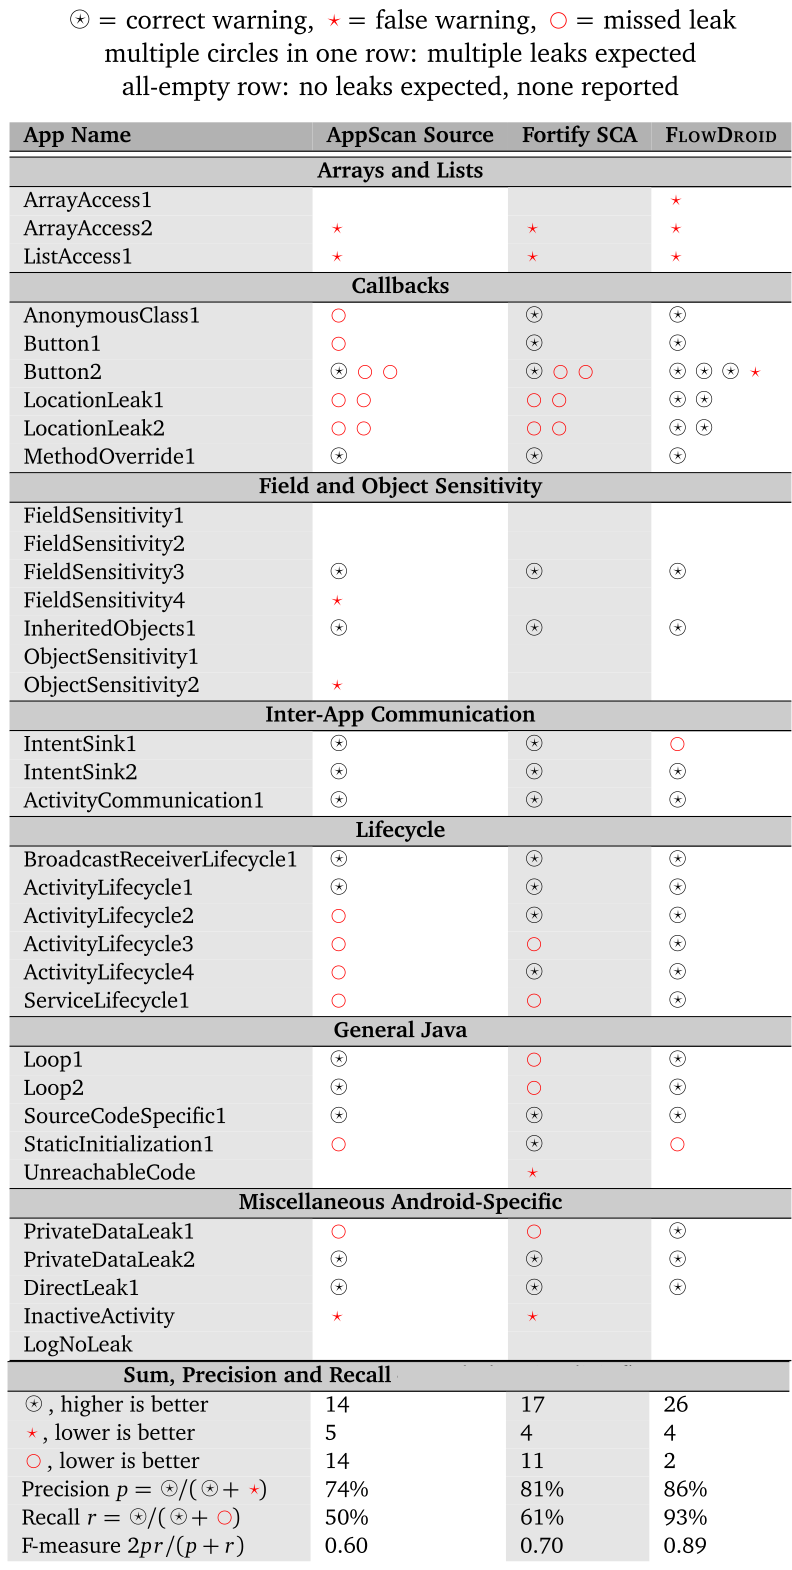
\includegraphics[scale=1]{img/evaluation.png}
\caption{DroidBench Evaluierung, aus \cite{technical}}
\label{fig:eval}
\end{figure} 
 
\section{Ausblick} 
FlowDroid macht viele richtig, aber wie die Evaluierung gezeigt hat, ist FlowDroid noch nicht perfekt. 
\\Zum Einen sollte die Inter-App-Kommunikation verbessert werden, damit auch tainted Daten zwischen den Komponenten verfolgt werden können. Dazu könnte der Sink der einen Komponente gleichzeitig die Source der anderen Komponenten sein.
Zum Anderen hat FlowDroid keine Sanitization implementiert. Dies ist jedoch notwendig, damit der Programmierer auf gefundene Fehler reagieren kann. 
Für die Zukunft wäre es auch wichtig, dass FlowDroid unterscheiden kann zwischen notwendigen und bösartigen Datenlecks. Eine Navigationsapp benötigt den Benutzerstandort. Eine Taschenlampen App jedoch nicht.
\\Schließlich wäre es auch hilfreich, wenn die Analyse für bestimmte Arten von Sinks und Sources einschränkbar wäre. Der Vorteil hierbei wäre, dass man sich bestimmte Datenflüsse näher anschauen könnte. SuSi klassifiziert und kategoriesiert bereits die Sinks und Sources.
% Normaler LNCS Zitierstil
%\bibliographystyle{splncs}
 
\nocite{*}
\bibliographystyle{plain}
\bibliography{literatur}
\end{document}
